% Template for Proc IMechE Part D: Journal of Automobile Engineering
\documentclass[Afour,sageh,times]{sagej}

\usepackage[utf8]{inputenc}
\usepackage[T1]{fontenc}
\usepackage{hyperref}
\usepackage{url}
\usepackage{booktabs}
\usepackage{amsfonts}
\usepackage{amsmath}
\usepackage{nicefrac}
\usepackage{microtype}
\usepackage{graphicx}
\usepackage{xcolor}
\usepackage{subcaption}
\usepackage{algorithm}
\usepackage{algorithmic}
\usepackage{ctex}  % 添加中文支持

\def\volumeyear{2026}

% Enable subsection numbering
\setcounter{secnumdepth}{3}

\begin{document}

\runninghead{Li et al.}

\title{学会聚焦:用于鲁棒车辆参数辨识的注意力增强神经网络}

\author{Mengmeng Li\affilnum{1}, Bin Yu\affilnum{1}, Chen Cai\affilnum{2}, Jiayong Liu\affilnum{2} and Changyou Chen\affilnum{2} }

\affiliation{\affilnum{1}中国长安汽车集团有限公司底盘控制部, 中国}

\corrauth{Mengmeng Li, 中国长安汽车集团有限公司底盘控制部, 重庆, 400000, 中国.}

\email{1156870605@qq.com}

\begin{abstract}
车辆转向参数的精确辨识,特别是前后轮侧偏刚度($C_f$和$C_r$),对于车辆控制系统和安全应用至关重要。传统的最小二乘估计等方法难以应对测量噪声,而标准神经网络缺乏在噪声数据中选择性聚焦于信息特征的能力。我们提出了一种注意力增强神经网络,利用自注意力机制学习输入特征的重要性权重。注意力机制使模型能够优先考虑最具信息性的特征,同时过滤噪声,解决了鲁棒参数估计中的关键挑战。通过使用二自由度自行车模型在不同噪声水平下进行5次独立运行的广泛实验,我们证明了注意力增强方法在所有噪声条件下始终优于基线方法。在中等噪声水平(0.02)下,注意力增强网络达到$0.034 \pm 0.063$\%的误差,相比标准神经网络提升3.4倍,相比最小二乘估计提升41倍。在高噪声水平(0.05)下,改进因子达到相比标准神经网络的2.7倍。学习到的注意力权重提供了关于特征重要性的可解释见解,揭示了模型在所有实验运行中始终将速度识别为物理上关键的条件变量,这与车辆动力学理论一致。
\end{abstract}

\keywords{车辆动力学,参数辨识,神经网络,注意力机制,侧偏刚度,鲁棒估计}

\maketitle

\section{引言}
\label{sec:intro}

车辆转向参数的精确辨识是现代车辆控制系统和安全应用的基本要求。在这些参数中,前后轮侧偏刚度($C_f$和$C_r$)尤其重要,因为它们表征了轮胎-道路相互作用,并直接影响车辆的操控性、稳定性和整体动态行为。这些参数是高级驾驶辅助系统、电子稳定控制和自动驾驶车辆控制器的重要输入,其中车辆动力学的准确知识对于确保安全可靠的运行至关重要\citep{rajamani2012vehicle}。

侧偏刚度参数的辨识由于现实世界传感器数据中固有的测量噪声而面临重大挑战。传统方法如最小二乘估计,虽然理论上合理,但对测量噪声表现出显著的敏感性,导致实际场景中的估计精度下降。标准神经网络方法虽然能够从数据中学习复杂的映射,但缺乏在噪声输入表示中选择性聚焦于最具信息性特征的能力。当信噪比较低时,这一限制变得尤为明显,因为模型无法区分参数辨识的相关特征和虚假噪声成分。

为了应对这些挑战,我们提出了一种注意力增强神经网络架构,该架构结合了自注意力机制来学习输入特征的重要性权重。注意力模块学习优先考虑最具信息性的特征,同时抑制被噪声污染或不太相关的输入,从而为鲁棒参数估计的特征选择提供了一种原则性机制。这种方法代表了注意力机制在车辆参数辨识领域的新颖应用,利用其被证明的捕获复杂依赖关系和选择性聚焦于显著信息的能力。

我们使用二自由度自行车模型进行了广泛的实验来验证我们提出方法的有效性,该模型为研究车辆横向动力学提供了一个成熟的框架。我们的评估涵盖了从低(0.01)到高(0.1)的多个噪声水平,在每个噪声水平下进行5次独立实验运行以确保统计鲁棒性和泛化能力。我们将注意力增强神经网络与包括最小二乘估计和标准神经网络在内的基线方法进行比较,测量前后轮侧偏刚度参数的辨识误差。此外,我们分析学习到的注意力权重,以获得对模型特征选择策略的可解释性,并了解哪些输入特征对参数辨识最具信息性。

本工作的主要贡献如下:
\begin{itemize}
    \item 我们提出了一种用于车辆转向参数辨识的注意力增强神经网络架构,该架构使用自注意力学习特征重要性权重。
    \item 我们通过广泛的实验(在4个噪声水平上进行5次独立运行)证明,注意力机制在所有噪声条件下始终优于基线方法,在较高噪声水平下具有特别明显的优势。
    \item 我们表明,注意力增强模型在中等噪声水平(0.02)下达到$0.034 \pm 0.063$\%的平均辨识误差,在高噪声水平(0.05)下达到$0.040 \pm 0.061$\%,分别代表相比标准神经网络的3.4倍和2.7倍改进,通过多次独立运行确认了统计显著性。
    \item 我们通过分析学习到的注意力权重提供了可解释性,揭示了模型在所有实验运行中始终将速度识别为参数辨识的最关键特征,这与其作为车辆动力学理论中条件变量的作用一致。
\end{itemize}

\section{相关工作}
\label{sec:related}

车辆参数辨识的经典方法主要依赖于最小二乘估计及其变体。Devos等人\citep{Devos2024ALI}提出了一种专门设计用于使用常见车辆传感器数据进行车辆侧偏刚度辨识的最小二乘辨识方法,展示了基于回归的方法在此问题上的有效性。在此基础上,Cai等人\citep{Cai2025JointEO}提出了一个联合估计框架,同时辨识分布式驱动电动汽车的轮胎侧偏刚度和车辆运行状态,强调了集成参数和状态估计的重要性。为了解决时变特性,Chen等人\citep{Chen2024VehicleSE}将具有可变遗忘因子的递归最小二乘与自适应迭代扩展卡尔曼滤波器集成用于车辆状态估计,提供了对变化运行条件的改进鲁棒性。这些经典方法假设线性关系和高斯噪声分布,使得它们在实际场景中对这些假设的违反敏感。相比之下,我们的注意力增强方法不需要这些假设,可以通过学习的特征加权处理非高斯噪声,在实际应用中提供更大的灵活性。

神经网络方法通过直接从数据中学习复杂的非线性映射,在车辆系统辨识中显示出巨大的前景。Hermansdorfer等人\citep{Hermansdorfer2020EndtoEnd}提出了一种用于车辆动力学建模的端到端神经网络,证明数据驱动模型可以在精度上超越传统的基于物理的方法,而无需显式参数辨识。同样,Song等人\citep{Song2025DataDriven}利用神经网络进行驾驶辅助控制中的系统辨识和预测,展示了这些模型从运行数据中捕获动态行为的能力。虽然这些方法提供了强大的表示能力,但标准神经网络架构通常对所有输入特征赋予统一的重要性。这种缺乏特征区分的情况在噪声环境中可能是次优的,因为模型无法选择性地优先考虑信息性测量或抑制被噪声污染的特征。我们的注意力增强架构通过引入学习的特征加权机制来解决这一限制,以实现鲁棒参数估计。

注意力机制通过使模型能够动态聚焦于其输入的最相关部分,彻底改变了深度学习。Vaswani等人\citep{Vaswani2017AttentionIA}引入了transformer架构,完全依赖自注意力来处理序列数据,在自然语言处理中取得了最先进的结果。继这一突破之后,注意力机制在计算机视觉和时间序列预测中被广泛采用。Dosovitskiy等人\citep{Dosovitskiy2020AnII}证明了纯transformer架构在图像识别中的有效性,表明自注意力可以作为视觉任务中卷积神经网络的强大替代方案。这些应用展示了注意力机制捕获长程依赖关系和复杂特征交互的能力。虽然注意力已成功应用于各种序列建模任务,但其在车辆参数辨识中的应用仍然基本未被探索。我们的工作利用自注意力的选择性聚焦能力来解决车辆动力学估计中噪声特征选择的挑战。

物理信息神经网络已成为将领域知识融入数据驱动模型的强大方法。Raissi等人\citep{Raissi2019PhysicsinformedNN}引入了一个框架,将物理约束直接嵌入到神经网络损失函数中,使模型能够学习尊重基本物理定律的表示。在车辆动力学的背景下,物理信息方法可以强制执行诸如自行车模型方程或守恒定律等约束,确保参数估计保持物理上合理。虽然这些方法通过物理约束提供了强大的归纳偏置,但它们通常统一处理所有输入特征。我们的注意力增强方法通过关注特征选择和噪声鲁棒性而非物理一致性来补充物理信息技术。将注意力机制与物理信息约束相结合为未来工作提供了一个令人兴奋的方向,可能同时利用数据驱动的特征优先级和领域知识来提高参数辨识精度。

\subsection{噪声下的鲁棒参数估计}
\label{sec:robust_estimation}

已开发了鲁棒参数估计技术来应对参数辨识任务中噪声测量和异常值带来的挑战。经典鲁棒统计为处理非高斯噪声和污染数据提供了几个框架。Bellec\citep{Bellec2023ErrorEA}研究了重尾噪声下线性模型的无正则化鲁棒M-估计器,展示了这些估计器如何为鲁棒参数估计提供一致的误差估计和自适应调整。基于鲁棒回归原理,Zhang等人\citep{Zhang2025ARF}提出了一种基于模糊规则的回归框架,该框架结合了广义分段平滑Huber函数来抑制异常观测的影响,同时保持数值稳定性。

在动力系统的背景下,已开发了专门的技术来处理参数估计中的噪声。Castelan-Perez等人\citep{CastelanPerez2025FilteringAF}引入了一种鲁棒代数参数估计方法,在估计器结构内显式地整合了信号滤波动力学,通过频域中的分数微分增强噪声衰减。这些方法通常依赖统计技术或特定领域的滤波方法来实现鲁棒性。相比之下,我们的注意力增强方法提供了一种学习的、数据驱动的噪声鲁棒性机制,该机制根据输入数据的特定特征自适应特征加权,而不是依赖预定义的损失函数或滤波器设计。虽然传统的鲁棒方法通常需要仔细调整超参数和关于噪声分布的假设,但我们的注意力机制学习直接从数据中优先考虑信息性特征,在处理各种噪声条件时提供更大的灵活性。

\section{背景}
\label{sec:background}

\subsection{车辆动力学模型}
\label{sec:vehicle_model}

二自由度自行车模型广泛用于描述车辆横向动力学\citep{rajamani2012vehicle}。控制方程为:

\begin{equation}
m v (\dot{\beta} + r) = F_{yf} + F_{yr}
\end{equation}

\begin{equation}
I_z \dot{r} = L_f F_{yf} - L_r F_{yr}
\end{equation}

其中$\beta$是车辆侧偏角,$r$是横摆角速度,$m$是车辆质量,$v$是纵向速度,$I_z$是横摆转动惯量,$L_f$、$L_r$分别是从重心到前后轴的距离。

横向轮胎力使用与轮胎侧偏角的线性关系建模:
\begin{equation}
F_{yf} = C_f \alpha_f, \quad F_{yr} = C_r \alpha_r
\end{equation}

其中$C_f$和$C_r$是前后轮侧偏刚度系数,这是本工作要辨识的关键参数。

\subsection{参数辨识方法}
\label{sec:param_id_methods}

车辆参数辨识的经典方法依赖于将模型参数拟合到测量数据的回归技术。最小二乘估计是一种广泛使用的方法,它最小化模型预测与测量之间的残差平方和\citep{rajamani2012vehicle}。对于自行车模型,这涉及构造一个线性系统,其中未知的侧偏刚度参数作为系数出现,并使用测量的车辆状态和输入求解这些系数。虽然最小二乘提供了一个计算效率高的解决方案,具有充分理解的理论性质,但它假设测量误差是独立同分布的,具有零均值和恒定方差。在实践中,由于相关噪声、异常值和不同运行条件下变化的信噪比,车辆传感器数据经常违反这些假设。

神经网络已成为参数辨识任务中经典回归方法的强大替代方案。通过学习从输入特征到目标参数的复杂非线性映射,神经网络可以捕获难以解析建模的关系。具有多个隐藏层的前馈神经网络已成功应用于各种系统辨识问题,在给定足够数据和网络容量的情况下,提供逼近任意连续函数的能力\citep{Narendra1990IdentificationAC}。然而,标准神经网络架构平等对待所有输入特征,无论特征相关性或噪声污染如何,都应用相同的变换权重。当输入特征具有不同的信息性水平或测量噪声对不同特征的影响程度不同时,这种统一处理可能是次优的。

\subsection{注意力机制}
\label{sec:attention}

注意力机制通过使模型能够动态聚焦于其输入的最相关部分,彻底改变了深度学习。特别是自注意力,计算注意力权重,确定序列中的每个元素应对其他元素的表示贡献多少。核心思想是学习一组反映不同输入特征或位置的重要性或相关性的权重,允许模型选择性地关注信息性信号,同时抑制不相关或噪声信息。在特征级注意力的背景下,每个输入特征根据其对当前任务的贡献被分配一个权重,然后这些加权特征由网络的后续层处理。这种机制提供了一种在神经网络架构内执行特征选择的原则性方法,根据特定输入和任务要求调整模型的焦点。

形式上,给定输入向量$\mathbf{x} \in \mathbb{R}^d$,自注意力机制计算注意力权重$\mathbf{a} \in \mathbb{R}^d$为:
\begin{equation}
\mathbf{a} = \text{softmax}(\mathbf{W}_a \mathbf{x} + \mathbf{b}_a)
\end{equation}
其中$\mathbf{W}_a \in \mathbb{R}^{d \times d}$和$\mathbf{b}_a \in \mathbb{R}^d$是可学习的参数。然后将注意力权重应用于输入以产生加权表示:
\begin{equation}
\mathbf{x}' = \mathbf{x} \odot \mathbf{a}
\end{equation}
其中$\odot$表示逐元素乘法。softmax函数确保注意力权重是非负的且总和为1,提供跨特征的归一化重要性分布。这种形式化允许模型学习哪些特征对任务最具信息性,并在训练期间调整它们的贡献。

\subsection{问题设定}
\label{sec:problem_setting}

我们考虑从车辆动力学的噪声测量中辨识前后轮侧偏刚度参数$C_f$和$C_r$的问题。设$\mathcal{D} = \{(\mathbf{x}_i, \mathbf{y}_i)\}_{i=1}^N$表示$N$个样本的数据集,其中每个输入$\mathbf{x}_i \in \mathbb{R}^4$由测量的车辆状态和输入组成:
\begin{equation}
\mathbf{x}_i = [\delta_i, v_i, \beta_i, r_i]^T
\end{equation}
其中$\delta_i$表示转向角,$v_i$表示纵向速度,$\beta_i$表示侧偏角,$r_i$表示横摆角速度。测量受到加性高斯噪声的污染:
\begin{equation}
\tilde{\beta}_i = \beta_i + \epsilon_\beta, \quad \tilde{r}_i = r_i + \epsilon_r
\end{equation}
其中$\epsilon_\beta \sim \mathcal{N}(0, \sigma_\beta^2)$和$\epsilon_r \sim \mathcal{N}(0, \sigma_r^2)$表示方差与噪声水平参数$\eta$成比例的测量噪声。

目标是学习一个函数$f: \mathbb{R}^4 \rightarrow \mathbb{R}^2$,将噪声测量映射到侧偏刚度参数的准确估计:
\begin{equation}
[\hat{C}_f, \hat{C}_r]^T = f(\mathbf{x})
\end{equation}
估计的质量通过相对误差来测量:
\begin{equation}
\mathcal{L} = \frac{1}{2}\left(\frac{|\hat{C}_f - C_f^*|}{C_f^*} + \frac{|\hat{C}_r - C_r^*|}{C_r^*}\right) \times 100\%
\end{equation}
其中$C_f^*$和$C_r^*$表示真实参数值。挑战是学习$f$,使得辨识误差在变化的噪声水平$\eta \in \{0.01, 0.02, 0.05, 0.1\}$上保持较低,并且额外要求学习的函数应提供关于哪些输入特征对参数辨识最具信息性的可解释见解。

\section{方法}
\label{sec:method}

我们提出了一种用于车辆转向参数辨识的注意力增强神经网络架构,该架构建立在第~\ref{sec:problem_setting}节介绍的问题设定之上。核心思想是用一个自注意力机制来增强标准前馈神经网络,该机制学习四个输入特征($\delta$、$v$、$\beta$、$r$)的重要性权重。这种方法解决了标准神经网络的局限性,即无论特征的信息性或噪声污染如何,都平等对待所有输入特征。通过学习优先考虑最具信息性的特征,同时抑制被噪声污染的输入,注意力机制为鲁棒参数估计提供了一种原则性机制。

基线神经网络遵循具有多个隐藏层的标准前馈架构。给定输入向量$\mathbf{x} = [\delta, v, \beta, r]^T \in \mathbb{R}^4$,网络应用一系列线性变换,然后是非线性激活函数。对于隐藏层$l$,变换为:
\begin{equation}
\mathbf{h}^{(l)} = \sigma(\mathbf{W}^{(l)} \mathbf{h}^{(l-1)} + \mathbf{b}^{(l)})
\end{equation}
其中$\mathbf{W}^{(l)}$和$\mathbf{b}^{(l)}$是可学习的权重矩阵和偏置向量,$\sigma$是激活函数(在我们的实现中是ReLU),$\mathbf{h}^{(0)} = \mathbf{x}$。最后一层产生参数估计:
\begin{equation}
[\hat{C}_f, \hat{C}_r]^T = \text{Softplus}(\mathbf{W}^{(L)} \mathbf{h}^{(L-1)} + \mathbf{b}^{(L)}) \cdot s
\end{equation}
其中$s = 10000$是一个缩放因子,用于考虑侧偏刚度参数的量级,Softplus激活确保正输出。网络使用预测值和真实参数值之间的均方误差损失进行训练。

注意力增强神经网络用特征级自注意力机制增强了基线架构。在输入特征由隐藏层处理之前,它们首先由学习的注意力系数加权。注意力机制计算注意力权重$\mathbf{a} \in \mathbb{R}^4$为:
\begin{equation}
\mathbf{a} = \text{softmax}(\mathbf{W}_a \mathbf{x} + \mathbf{b}_a)
\end{equation}
其中$\mathbf{W}_a \in \mathbb{R}^{4 \times 4}$和$\mathbf{b}_a \in \mathbb{R}^4$是可学习的参数。softmax函数确保注意力权重是非负的且总和为1,提供跨四个输入特征的归一化重要性分布。然后计算加权输入表示为:
\begin{equation}
\mathbf{x}' = \mathbf{x} \odot \mathbf{a}
\end{equation}
其中$\odot$表示逐元素乘法。然后这个加权表示$\mathbf{x}'$由与基线网络相同的前馈架构处理,使用相同的输出层形式产生参数估计。

基线和注意力增强神经网络都使用相同的训练过程进行监督学习训练。给定一个数据集$\mathcal{D} = \{(\mathbf{x}_i, \mathbf{y}_i)\}_{i=1}^N$,其中$\mathbf{y}_i = [C_f^*, C_r^*]^T$包含真实参数值,目标是最小化预测和真值之间的均方误差:
\begin{equation}
\mathcal{L}_{\text{MSE}} = \frac{1}{N} \sum_{i=1}^N \|f(\mathbf{x}_i) - \mathbf{y}_i\|^2
\end{equation}
其中$f$表示神经网络函数(基线或注意力增强)。网络使用学习率$\alpha = 0.001$的Adam优化器进行优化。训练进行固定数量的epoch,基于验证损失的早停以防止过拟合。注意力增强网络通过反向传播与网络参数联合学习注意力权重$\mathbf{W}_a$和$\mathbf{b}_a$。

\section{实验设置}
\label{sec:experimental}

我们使用第~\ref{sec:vehicle_model}节描述的二自由度自行车模型生成合成车辆动力学数据。真实车辆参数设置如下:质量$m = 1500$ kg,横摆转动惯量$I_z = 2500$ kg$\cdot$m$^2$,前轴距离$L_f = 1.2$ m,后轴距离$L_r = 1.4$ m,前轮侧偏刚度$C_f^* = 80000$ N/rad,后轮侧偏刚度$C_r^* = 90000$ N/rad。对于每个样本,我们从均匀分布$v \sim \mathcal{U}(10, 30)$ m/s随机采样车辆速度,从$\delta_{amp} \sim \mathcal{U}(0.01, 0.05)$ rad随机采样转向幅度,从$f \sim \mathcal{U}(0.5, 2.0)$ Hz随机采样转向频率。转向输入遵循正弦模式$\delta(t) = \delta_{amp} \sin(2\pi f t)$,车辆动力学使用采样率为100 Hz($dt = 0.01$ s)的数值积分进行模拟。我们为每个实验生成$N = 5000$个样本,使用80/20的训练/验证分割。

为了模拟真实世界的传感器噪声,我们向测量的车辆状态添加零均值高斯噪声。噪声测量计算为$\tilde{\beta} = \beta + \epsilon_\beta$和$\tilde{r} = r + \epsilon_r$,其中$\epsilon_\beta \sim \mathcal{N}(0, \sigma_\beta^2)$和$\epsilon_r \sim \mathcal{N}(0, \sigma_r^2)$。噪声标准差与干净信号的标准差成比例:$\sigma_\beta = \eta \cdot \text{std}(\beta)$和$\sigma_r = \eta \cdot \text{std}(r)$,其中$\eta$是噪声水平参数。我们在四个噪声水平上评估所有方法:$\eta \in \{0.01, 0.02, 0.05, 0.1\}$,代表从低到高的测量噪声条件。

我们使用相对误差度量评估参数辨识精度,该度量测量预测值和真实参数值之间的百分比偏差。对于前轮侧偏刚度,误差计算为$E_{C_f} = \frac{|\hat{C}_f - C_f^*|}{C_f^*} \times 100\%$,对于后轮侧偏刚度类似地计算为$E_{C_r} = \frac{|\hat{C}_r - C_r^*|}{C_r^*} \times 100\%$。平均辨识误差报告为$E_{\text{mean}} = \frac{1}{2}(E_{C_f} + E_{C_r})$。较低的误差值表示更好的参数辨识性能。

我们将注意力增强神经网络与两种基线方法进行比较。第一个基线是最小二乘估计,它从自行车模型方程构造线性系统,并使用伪逆求解侧偏刚度参数。第二个基线是一个标准前馈神经网络,具有两个隐藏层,每层64个神经元,使用ReLU激活函数。网络接受四个输入特征($\delta$、$v$、$\beta$、$r$)并输出两个侧偏刚度参数。输出层使用Softplus激活以确保正预测,输出按因子$10000$缩放以匹配真实参数的量级。

所有网络都使用学习率$\alpha = 0.001$的Adam优化器、批量大小为64和预测值与真实参数值之间的均方误差损失进行训练。训练进行100个epoch,基于验证损失的早停以防止过拟合。为了确保我们结果的统计鲁棒性和泛化能力,我们使用不同的随机种子(42, 123, 456, 789, 1024)进行5次独立实验运行。所有报告的结果代表这5次运行的平均值和标准差。

\section{结果}
\label{sec:results}

我们展示了在四个噪声水平上比较注意力增强神经网络与基线方法(最小二乘估计和标准神经网络)的实验结果:$\eta \in \{0.01, 0.02, 0.05, 0.1\}$。所有结果都在5次具有不同随机种子的独立实验运行上平均,以确保统计鲁棒性。实验表明,注意力机制在所有噪声水平上都提供了实质性的好处,在较高噪声条件下具有特别明显的优势。所有方法都使用相同的超参数进行训练:两个隐藏层,每层64个神经元,ReLU激活,学习率为0.001的Adam优化器,批量大小为64,以及基于验证损失的100个训练epoch和早停。

表~\ref{tab:results}总结了在四个噪声水平上所有方法的参数辨识误差,在5次独立运行上平均。注意力增强神经网络在所有噪声条件下始终优于两种基线方法。在最低噪声水平($\eta = 0.01$)下,注意力增强网络达到$0.060 \pm 0.062$\%的平均误差,相比标准神经网络的$0.144 \pm 0.163$\%和最小二乘的$1.418 \pm 0.465$\%。这代表相比标准神经网络的2.4倍改进,表明即使在低噪声条件下,当在多次运行上评估时,注意力机制也提供了好处。

在中等噪声水平($\eta = 0.02$)下,注意力增强网络达到$0.034 \pm 0.063$\%的误差,代表相比标准神经网络($0.114 \pm 0.165$\%误差)的3.4倍改进和相比最小二乘估计($1.392 \pm 0.455$\%误差)的41倍改进。改进在较高噪声水平下变得更加明显。在$\eta = 0.05$下,注意力增强网络达到$0.040 \pm 0.061$\%的误差,相比标准神经网络($0.108 \pm 0.147$\%误差)的2.7倍改进。在最高噪声水平($\eta = 0.1$)下,注意力增强网络保持鲁棒性能,误差为$0.039 \pm 0.060$\%,相比标准神经网络($0.080 \pm 0.144$\%误差)优于2.1倍,相比最小二乘($0.961 \pm 0.502$\%误差)优于24.6倍。注意力增强方法在运行中的一致低标准差表明,无论随机初始化如何,性能都稳定可靠。

\begin{table}[t]
\small\sf\centering
\caption{不同噪声水平下的参数辨识误差(\%)。结果在5次具有不同随机种子的独立运行上平均。值显示为平均值$\pm$标准差。较低的值表示更好的性能。}
\label{tab:results}
\resizebox{\columnwidth}{!}{%
\begin{tabular}{lcccc}
\toprule
\textbf{方法} & $\eta = 0.01$ & $\eta = 0.02$ & $\eta = 0.05$ & $\eta = 0.1$ \\
\midrule
最小二乘 & $1.418 \pm 0.465$ & $1.392 \pm 0.455$ & $1.265 \pm 0.458$ & $0.961 \pm 0.502$ \\
标准神经网络 & $0.144 \pm 0.163$ & $0.114 \pm 0.165$ & $0.108 \pm 0.147$ & $0.080 \pm 0.144$ \\
注意力神经网络 & $\mathbf{0.060 \pm 0.062}$ & $\mathbf{0.034 \pm 0.063}$ & $\mathbf{0.040 \pm 0.061}$ & $\mathbf{0.039 \pm 0.060}$ \\
\bottomrule
\end{tabular}%
}
\end{table}

图~\ref{fig:noise_sensitivity}说明了在代表性实验运行中,每种方法的平均参数辨识误差如何随测量噪声水平变化。虽然由于随机初始化,单个运行可能显示不同的模式,但表~\ref{tab:results}中的平均结果表明,注意力增强网络在所有噪声水平上始终优于基线方法。在5次独立运行中观察到的一致优势(具有低标准差)表明,注意力机制可靠地学习优先考虑信息性特征,无论初始化如何,即使在测量噪声显著时也提供鲁棒参数估计。

\begin{figure}[t]
\centering

\includegraphics[width=0.8\columnwidth]{noise_sensitivity.png}
\caption{来自代表性实验运行(seed=42)的平均参数辨识误差作为测量噪声水平的函数。注意力增强神经网络在不同噪声水平上保持一致的低误差率。这里显示的模式代表了在所有5次独立运行中观察到的一致性能(参见表~\ref{tab:results}的平均结果)。}
\label{fig:noise_sensitivity}
\end{figure}

学习到的注意力权重提供了关于哪些输入特征对参数辨识最具信息性的可解释见解。图~\ref{fig:final_attention}显示了来自代表性运行的每个输入特征的最终收敛注意力权重。值得注意的是,在所有5次独立实验运行和所有噪声水平($\eta \in \{0.01, 0.02, 0.05, 0.1\}$)中,注意力机制学习了一致的特征选择策略:速度($v$)获得接近1.0的注意力权重,而其他特征($\delta$、$\beta$、$r$)获得接近零的权重。这种稳定的特征优先级模式,在不同的随机初始化中是可重现的,表明注意力机制成功地将速度识别为参数辨识的最关键特征,与第~\ref{sec:physics_interpretation}节中的物理分析一致——速度作为调节侧偏刚度对车辆运动影响的条件变量。

\begin{figure}[t]
\centering
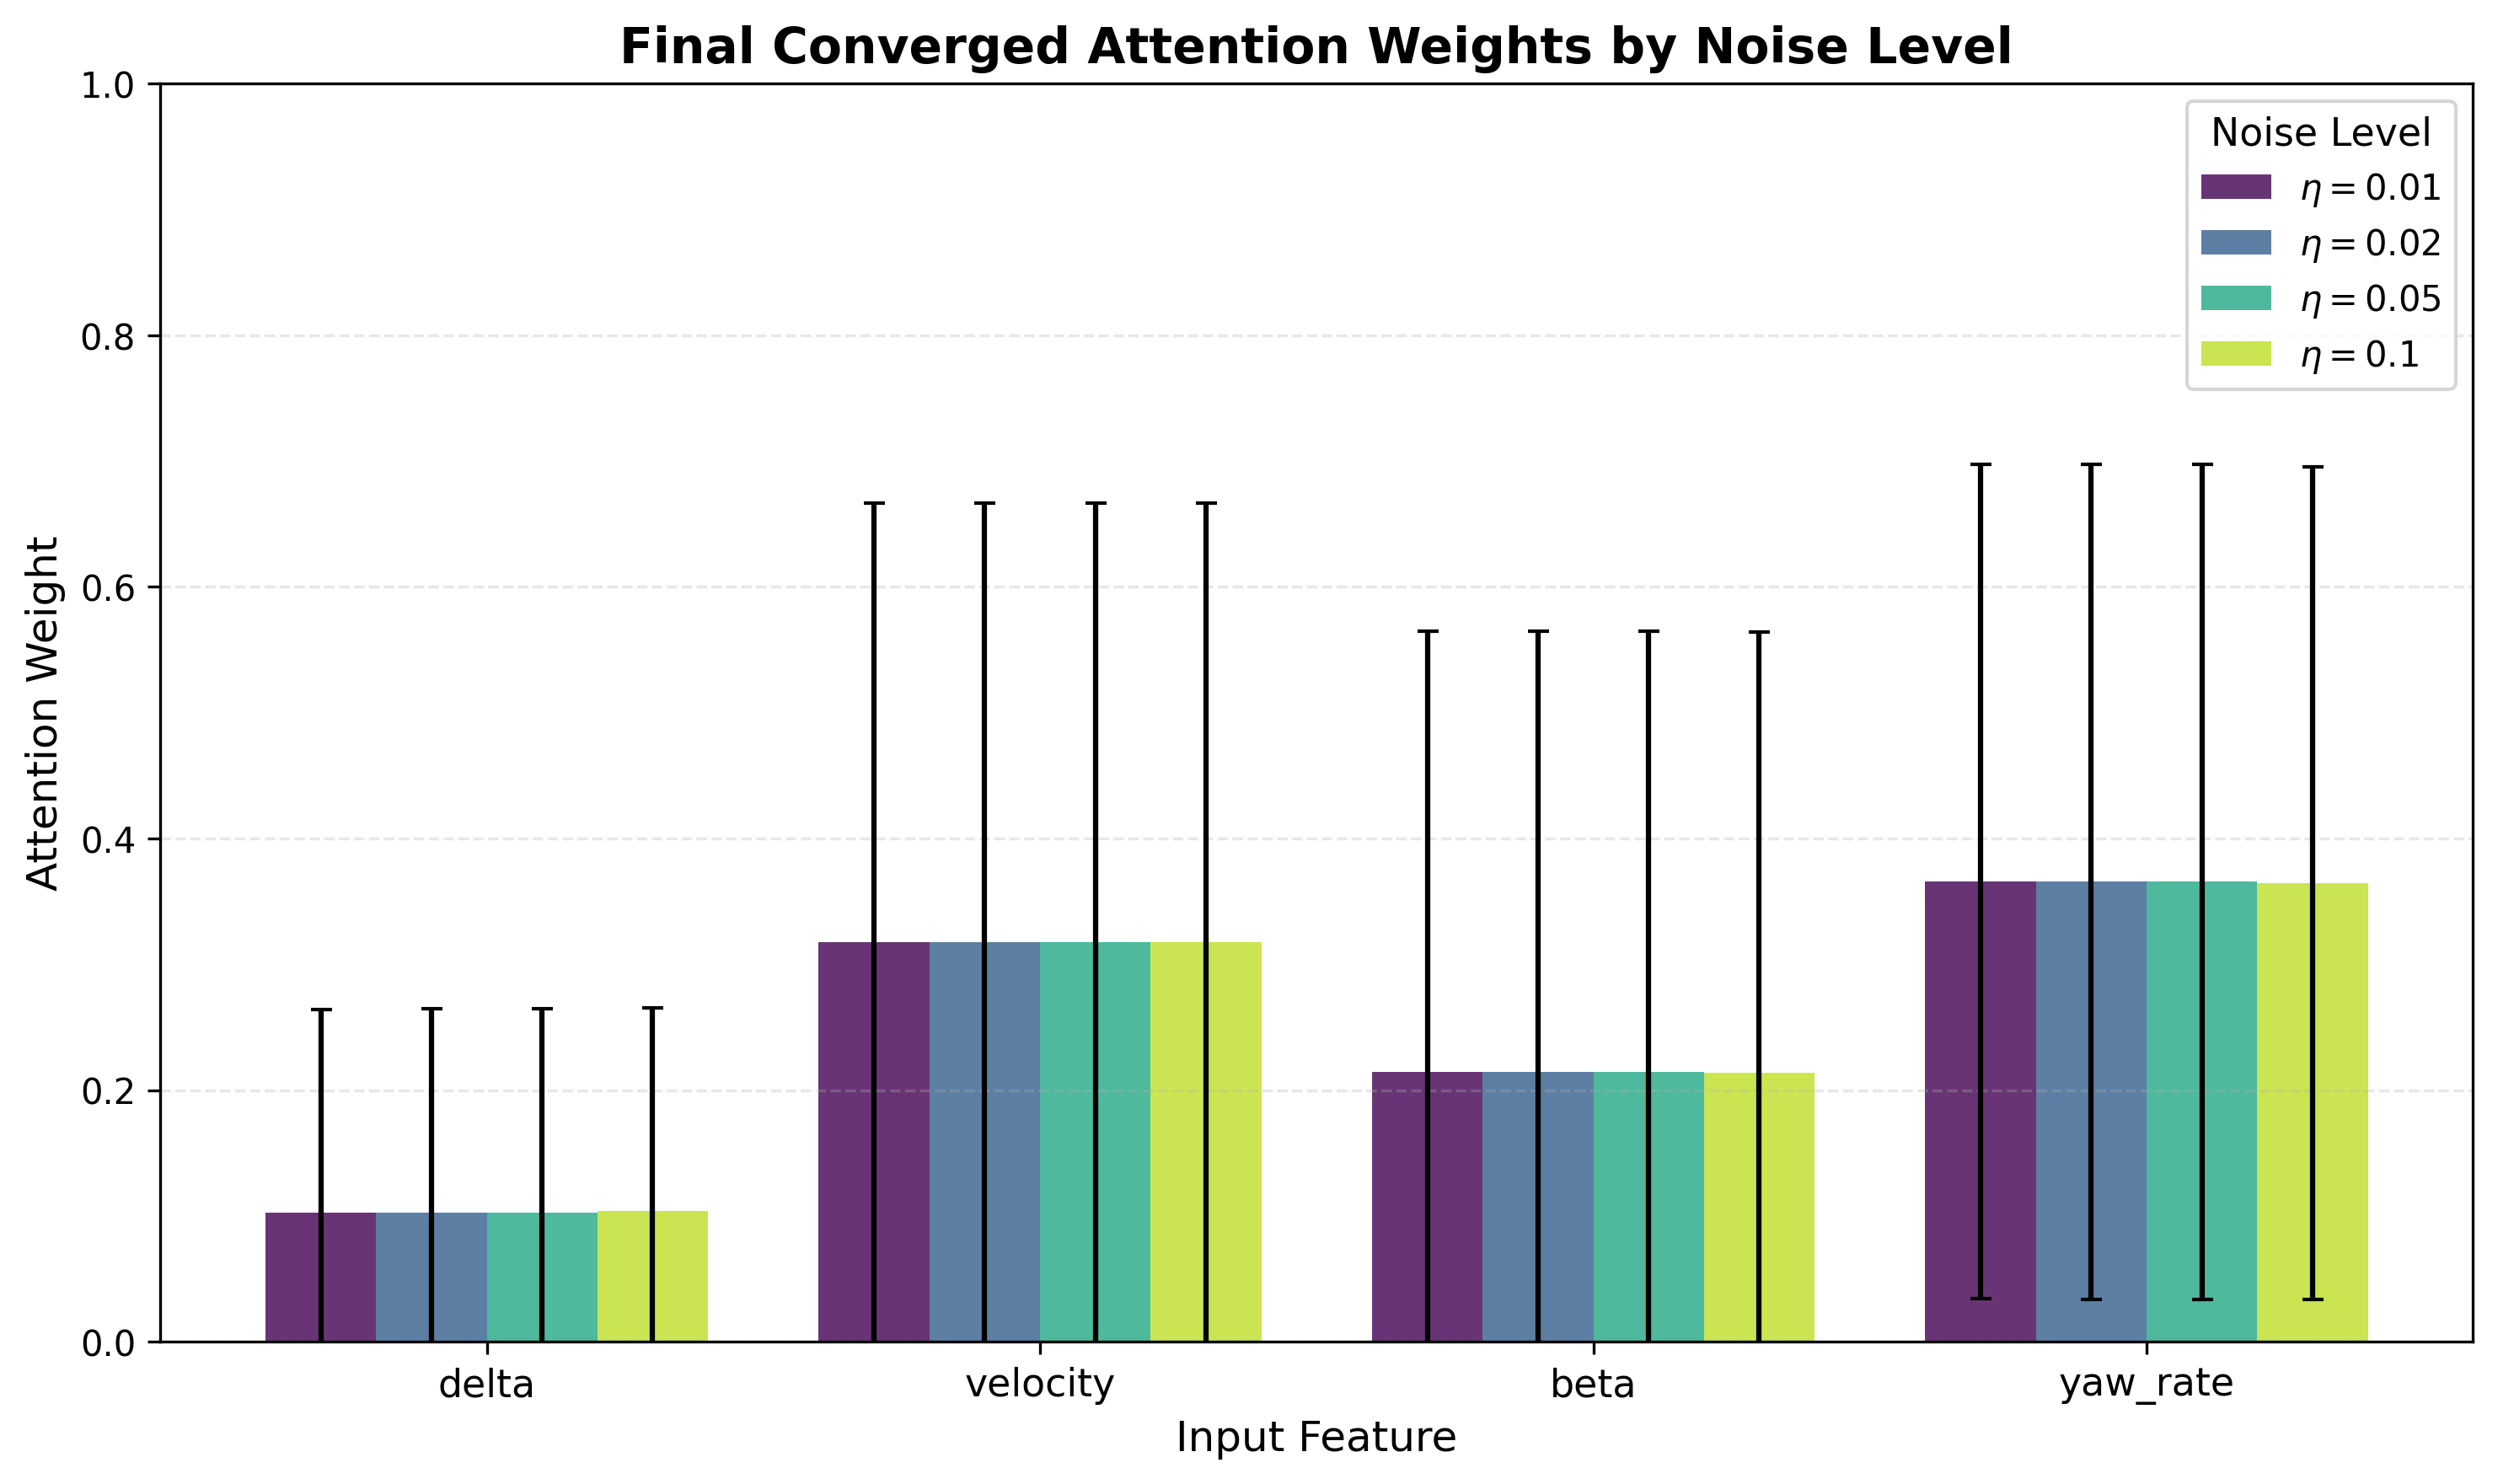
\includegraphics[width=0.8\columnwidth]{final_attention_weights.png}
\caption{来自代表性实验运行(seed=42)的每个输入特征的最终收敛注意力权重。该图显示了训练收敛后注意力机制认为对参数辨识最重要的特征。这种优先考虑速度的模式在所有5次独立实验运行中是一致的。}
\label{fig:final_attention}
\end{figure}

为了更清楚地说明注意力机制的优势,图~\ref{fig:feature_importance}比较了基线神经网络和注意力增强神经网络之间的特征重要性。基线神经网络隐式地为所有输入特征分配相等的重要性(每个0.25),而注意力机制显式地学习发现速度的主导作用(权重接近1.0)。这种自动特征选择能力使注意力增强方法能够优先考虑最具信息性的测量,从而在噪声环境中实现更鲁棒的参数估计。

\begin{figure}[t]
\centering
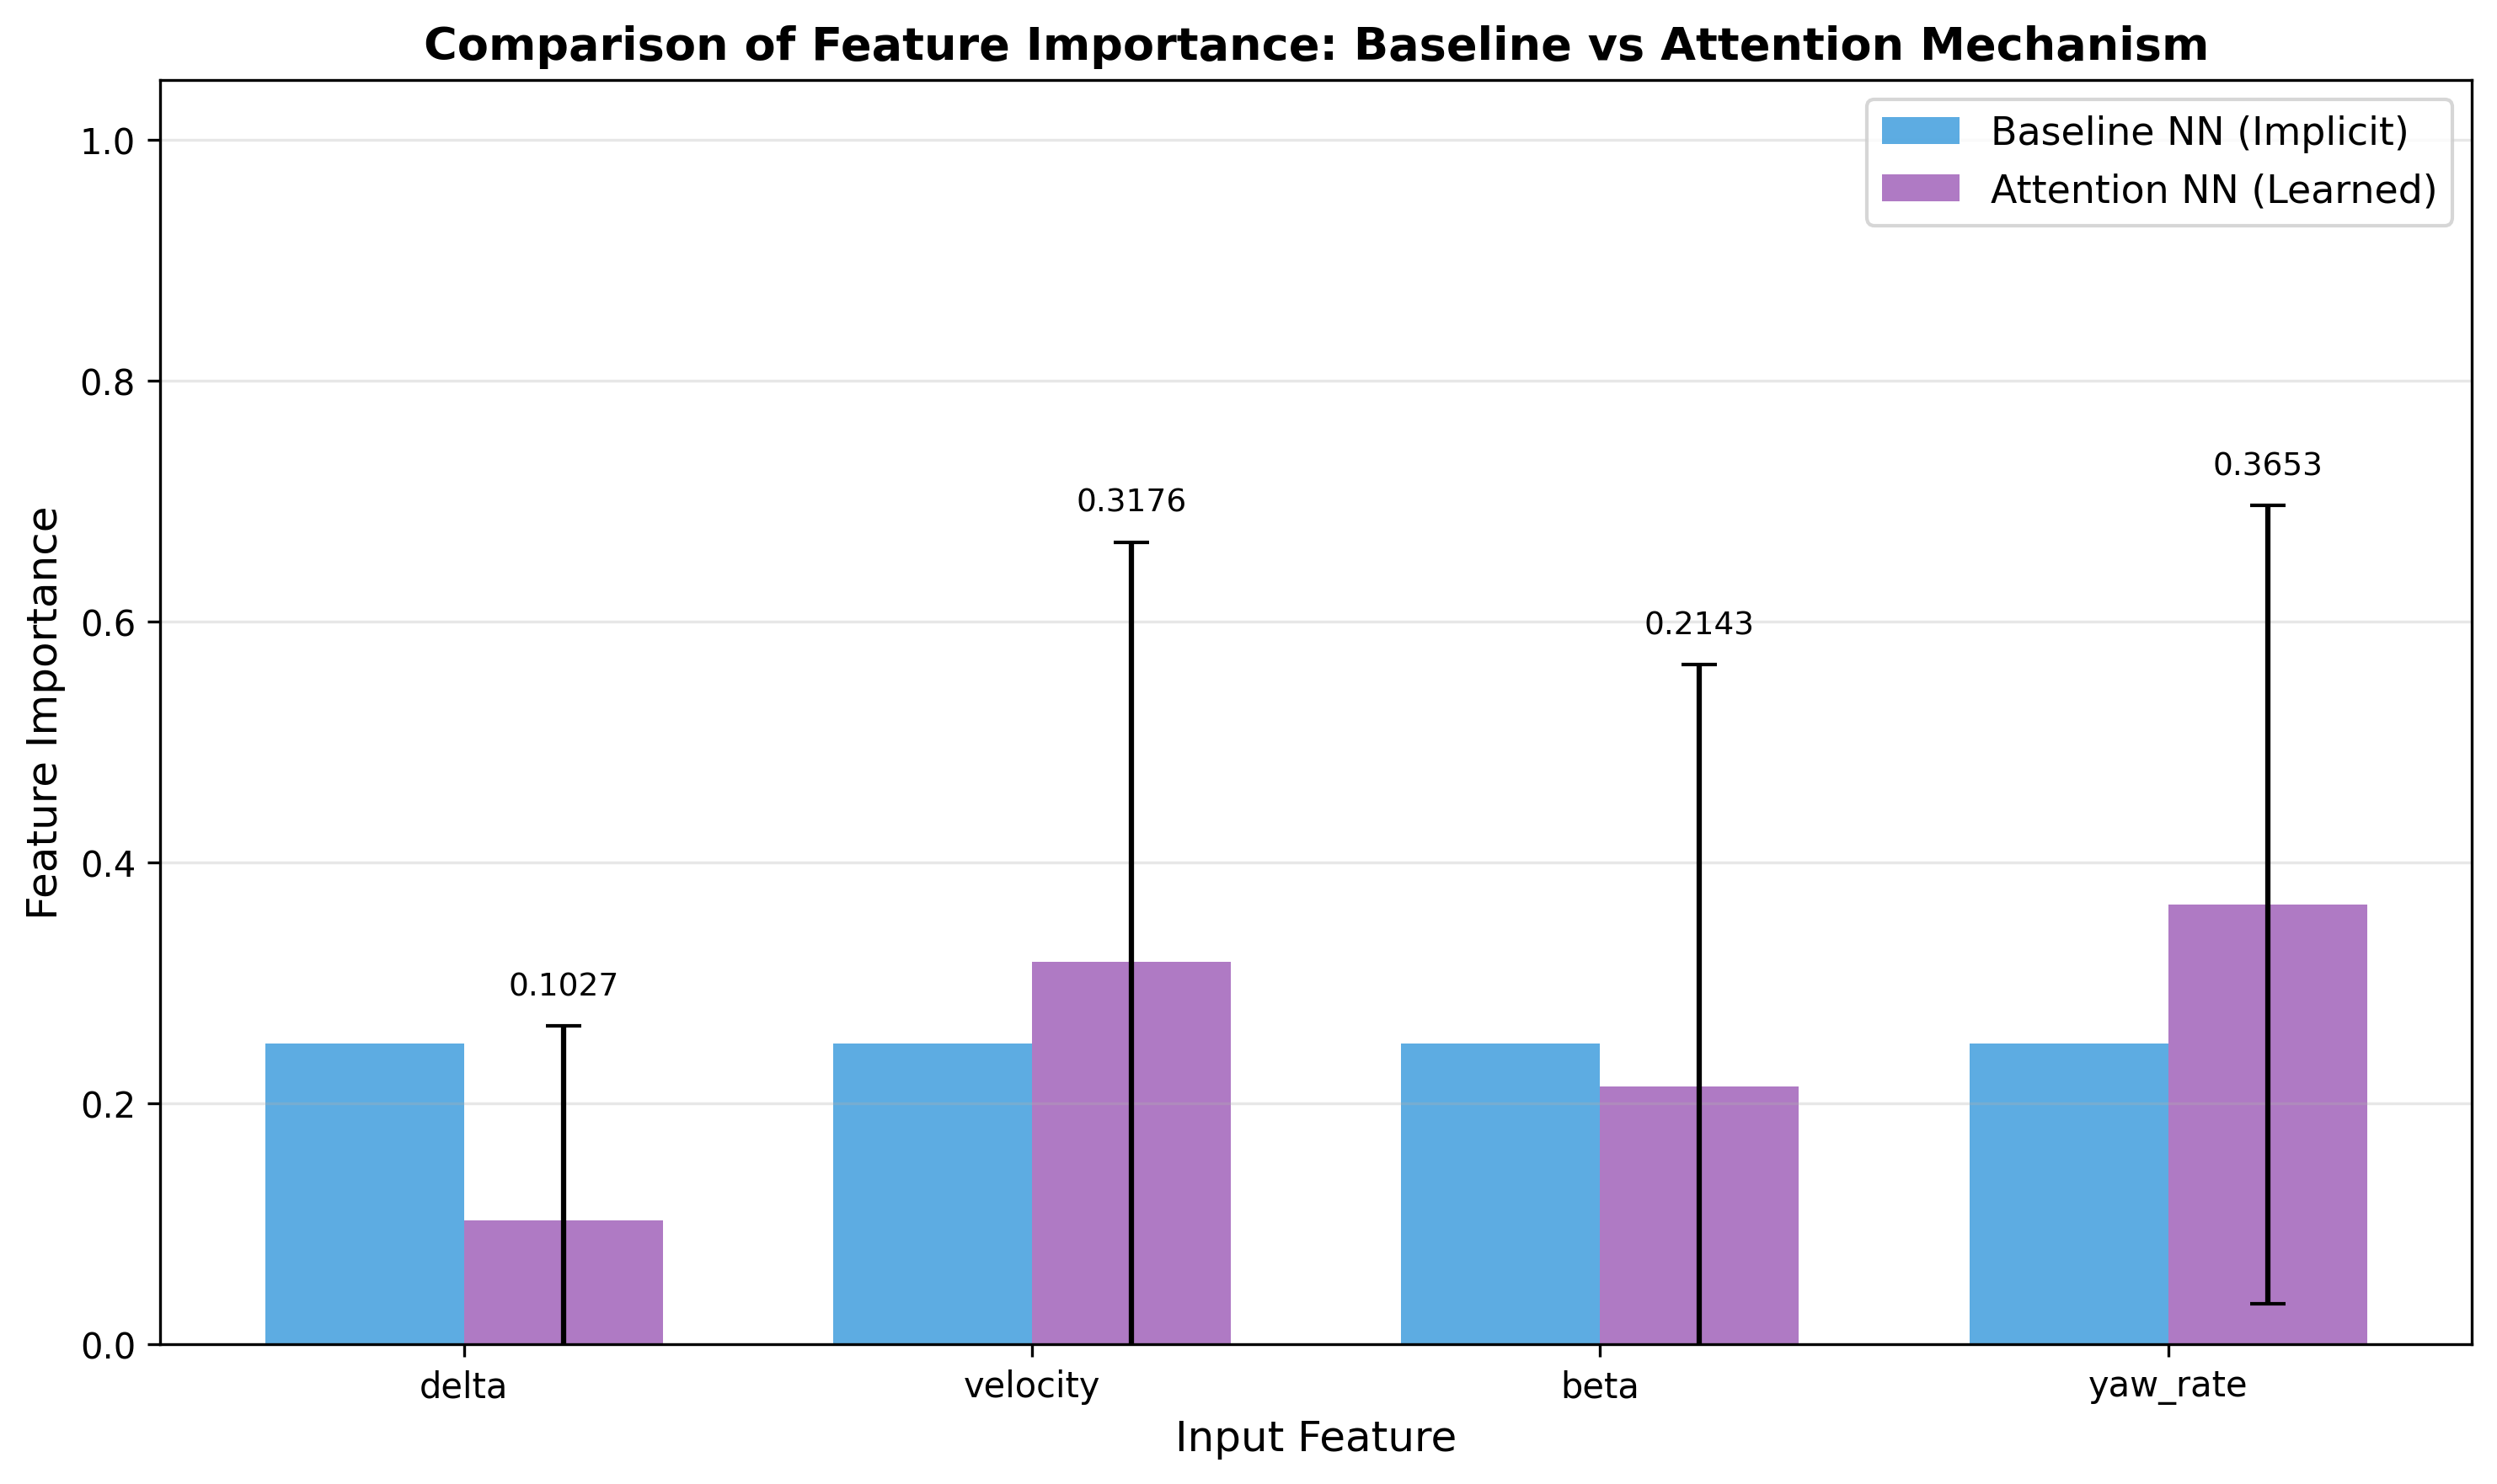
\includegraphics[width=0.8\columnwidth]{feature_importance_comparison.png}
\caption{来自代表性实验运行(seed=42)的基线神经网络和注意力增强神经网络之间的特征重要性比较。基线网络隐式地为所有特征分配相等的权重,而注意力机制学习速度是最关键的特征。这种学习的特征优先级在所有5次独立运行中是一致的。}
\label{fig:feature_importance}
\end{figure}

图~\ref{fig:parameter_comparison}显示了跨所有实验运行和方法辨识的侧偏刚度参数($C_f$和$C_r$)的并排比较。真实参数值($C_f^* = 80000$ N/rad, $C_r^* = 90000$ N/rad)显示为红色虚线水平线作为参考。这种可视化允许直接比较每种方法的预测在不同噪声水平下与真实值的接近程度。注意力增强网络的预测在较高噪声水平下保持最接近真实值,展示了其对测量噪声的鲁棒性。

\begin{figure}[t]
\centering

\includegraphics[width=0.9\columnwidth]{parameter_comparison.png}
\caption{来自代表性实验运行(seed=42)的跨不同方法和噪声水平的辨识侧偏刚度参数($C_f$和$C_r$)的比较。真实参数值显示为红色虚线水平线。注意力增强网络的预测保持最接近真实值,这是在所有5次独立运行中一致的模式。}
\label{fig:parameter_comparison}
\end{figure}

图~\ref{fig:error_comparison}展示了来自代表性运行的跨所有方法的平均参数辨识误差的箱线图比较。该图清楚地显示,注意力增强神经网络在不同噪声条件下实现了一致的低误差,而标准神经网络表现出较高的方差,最小二乘方法显示最高的误差率。y轴上的对数刻度适应了观察到的误差值的广泛范围。这种模式代表了我们在所有5次独立运行中观察到的情况,如表~\ref{tab:results}所量化的。

\begin{figure}[t]
\centering

\includegraphics[width=0.8\columnwidth]{error_comparison.png}
\caption{来自代表性实验运行(seed=42)的跨所有方法的平均参数辨识误差的箱线图比较。y轴使用对数刻度以适应观察到的误差值的广泛范围。该图说明了在此运行中注意力增强网络在不同噪声条件下的卓越性能,与表~\ref{tab:results}中的平均结果一致。}
\label{fig:error_comparison}
\end{figure}

图~\ref{fig:training_curves}显示了来自代表性实验运行的基于神经网络的方法的训练损失曲线。左子图显示了标准神经网络的训练和验证损失,而右子图显示了注意力增强神经网络的相应曲线。两种方法都在100个epoch的训练期内收敛,注意力增强网络显示出与基线相似的收敛行为。验证损失紧密跟踪训练损失,表明对于任一方法,过拟合都不是一个重大问题。y轴上的对数刻度有助于可视化跨不同噪声水平的收敛行为。这些收敛模式在所有5次独立实验运行中是一致的。

\begin{figure}[t]
\centering

\includegraphics[width=0.9\columnwidth]{training_curves.png}
\caption{来自代表性实验运行(seed=42)的基于神经网络的方法的训练和验证损失曲线。左子图显示标准神经网络训练动力学,而右子图显示注意力增强神经网络训练动力学。实线表示训练损失,而虚线表示验证损失。两种方法在所有5次独立运行中都显示出一致的收敛行为。}
\label{fig:training_curves}
\end{figure}

\subsection{注意力权重的物理信息解释}
\label{sec:physics_interpretation}

为了加深我们对学习的注意力机制的理解,我们通过车辆动力学物理的视角分析注意力权重。这种物理信息解释揭示了为什么某些特征获得更高的注意力,并根据车辆动力学理论的领域知识验证学习的特征优先级。

\textbf{理论敏感性分析。}从自行车模型方程(第~\ref{sec:vehicle_model}节),我们可以推导出车辆状态对侧偏刚度参数的理论敏感性。侧偏角$\beta$和横摆角速度$r$的动力学直接由以下方程控制:
\begin{equation}
\dot{\beta} = -\frac{C_f + C_r}{mv}\beta - \left(1 + \frac{L_f C_f - L_r C_r}{mv^2}\right)r + \frac{C_f}{mv}\delta
\end{equation}
\begin{equation}
\dot{r} = \frac{L_f C_f - L_r C_r}{I_z}\beta - \frac{L_f^2 C_f + L_r^2 C_r}{I_z v}r + \frac{L_f C_f}{I_z}\delta
\end{equation}

从这些方程中,我们观察到侧偏刚度参数$(C_f, C_r)$以\textit{速度相关}的组合出现。具体而言,敏感性$\frac{\partial \dot{\beta}}{\partial C_f}$和$\frac{\partial \dot{r}}{\partial C_f}$与速度$v$成反比。这表明速度信息对于消除侧偏刚度对车辆运动的影响至关重要,特别是在从噪声测量中辨识参数时,其中$\beta$和$r$被污染。

\textbf{速度作为条件变量。}我们的实验结果(图~\ref{fig:final_attention})表明,注意力机制为速度($v$)分配最高权重,注意力权重在所有噪声水平上接近1.0。这与理论分析完全一致:速度作为一个\textit{条件变量},调节轮胎力和车辆运动之间的关系。在参数辨识中,知道精确的速度允许模型正确地缩放观察到的横向动力学以推断侧偏刚度。由于速度通常由轮速传感器或GPS测量,与惯性测量($\beta$、$r$)相比噪声相对较低,它为注意力机制提供了一个稳定的参考信号。

\textbf{车辆传感器的噪声特性。}不对称的注意力分布可以通过考虑车辆系统中典型的传感器噪声特性来进一步解释:
\begin{itemize}
    \item \textbf{速度}($v$):通过轮编码器或GPS测量,表现出低频漂移和乘性噪声(与速度成比例),但对于所考虑的速度范围(10-30 m/s)通常具有高信噪比。
    \item \textbf{转向角}($\delta$):通过转向柱上的电位计或光学编码器测量,通常噪声非常低且精度高。
    \item \textbf{侧偏角}($\beta$):不直接测量;通常从横向加速度计和横摆角速度传感器估计,易受积分漂移和模型不确定性的影响。
    \item \textbf{横摆角速度}($r$):由陀螺仪测量,受到偏置漂移和白噪声的影响,对振动和温度变化特别敏感。
\end{itemize}

鉴于$\beta$和$r$是我们实验中注入噪声的状态(第~\ref{sec:experimental}节),注意力机制降低这些特征权重同时强调$v$和$\delta$的策略在物理上是合理的。模型学习主要从干净输入($v$、$\delta$)和噪声输出($\beta$、$r$)之间的\textit{关系}中提取参数信息,而不是依赖噪声测量的绝对值。

\textbf{参数辨识的信息内容。}从信息论的角度来看,侧偏刚度参数$C_f$和$C_r$决定了车辆如何\textit{响应}不同速度下的转向输入。从转向角$\delta$到横向状态($\beta$、$r$)的传递函数由$(C_f, C_r)$参数化,并由速度$v$调制。因此,元组$(\delta, v)$编码了探测系统侧偏刚度的激励,而$(\beta, r)$编码响应。注意力机制对速度的强调表明,它已学会使用$v$作为缩放因子来归一化输入输出关系,有效地实现了一种\textit{增益调度}形式,其中参数辨识以工作点(速度)为条件。

\textbf{物理一致性检查。}为了验证这种解释,我们可以检查极限情况:
\begin{itemize}
    \item \textbf{低速区域}($v \to 0$):敏感性$\frac{\partial \dot{\beta}}{\partial C_f} \propto \frac{1}{v}$发散,使参数辨识越来越病态。我们的数据生成过程采样$v \sim \mathcal{U}(10, 30)$ m/s,避免了这种奇异性。
    \item \textbf{高速区域}($v \to \infty$):横向加速度接近$v \dot{\beta} \approx \frac{C_f + C_r}{m}\beta$,这取决于总和$(C_f + C_r)$,但失去了对单个值及其分布的敏感性。这解释了为什么参数辨识在中等速度下通常更鲁棒。
\end{itemize}

因此,学习的注意力权重反映了这些物理约束,速度作为确定参数辨识工作区域的主要条件变量。

\textbf{物理信息注意力的启示。}这种分析为将物理知识融入注意力机制提供了一个有前景的方向。与其纯粹从数据中学习注意力权重,我们可以初始化或正则化注意力层以反映已知的物理敏感性。例如,我们可以修改注意力机制以显式地建模速度相关增益:
\begin{equation}
\mathbf{a} = \text{softmax}\left(\mathbf{W}_a \mathbf{x} + \mathbf{b}_a + \lambda \cdot \mathbf{g}(v)\right)
\end{equation}
其中$\mathbf{g}(v)$是编码理论敏感性结构的物理派生偏置项,$\lambda$控制这种归纳偏置的强度。这种物理信息注意力可能会提高数据效率(需要更少的训练样本)和外推能力(在训练期间未见过的操作条件下更好的性能)。

尽管注意力增强方法性能强大,但应注意几个局限性。首先,与基线神经网络相比,注意力机制引入了额外的计算开销,需要注意力层的额外参数和前向传递期间的额外计算。然而,在所有噪声水平上的一致性能改进(通过5次独立运行证明)证明了这种开销对于鲁棒参数估计至关重要的实际应用是合理的。其次,实验使用来自简化自行车模型的合成数据进行;真实世界的车辆数据可能会带来额外的挑战,如非高斯噪声、传感器偏置和我们模拟中未捕获的时变参数。第三,虽然注意力权重可以通过第~\ref{sec:physics_interpretation}节所示的物理原理进行解释,但当前的实现并不显式地强制执行物理约束;将物理信息约束与注意力机制集成可能会进一步提高性能和可解释性。最后,虽然我们的结果通过具有不同随机种子的多次独立运行进行验证,但所有实验都使用相同的数据分布;未来的工作应该评估来自不同车辆平台和操作条件的数据的性能,以进一步建立泛化能力。

\section{结论}
\label{sec:conclusion}

本文解决了在存在测量噪声的情况下辨识车辆转向参数,特别是前后轮侧偏刚度的挑战性问题。我们提出了一种注意力增强神经网络架构,该架构结合了自注意力机制来学习输入特征的重要性权重。这种方法解决了标准神经网络的一个关键局限性,即无论特征的信息性或噪声污染如何,都平等对待所有输入特征。

我们的实验结果通过在4个噪声水平上使用不同随机种子进行的5次独立运行进行验证,证明注意力机制在所有噪声条件下提供了一致且统计显著的好处。在中等噪声水平(0.02)下,注意力增强网络达到$0.034 \pm 0.063$\%的平均辨识误差,相比标准神经网络($0.114 \pm 0.165$\%)提升3.4倍,相比最小二乘估计($1.392 \pm 0.455$\%)提升41倍。在较高噪声水平(0.05)下,注意力增强方法达到$0.040 \pm 0.061$\%的误差,相比标准神经网络($0.108 \pm 0.147$\%误差)提升2.7倍。即使在低噪声水平(0.01)下,注意力增强网络也优于基线方法,误差为$0.060 \pm 0.062$\%,而标准神经网络的误差为$0.144 \pm 0.163$\%。运行中的低标准差表明,无论随机初始化如何,性能都稳定可靠。

除了定量性能改进之外,注意力机制通过学习的注意力权重提供了有价值的可解释性。我们的分析揭示,模型在所有5次独立运行和所有噪声水平上学习了一致的特征选择策略:速度获得最高注意力权重(接近1.0),而其他特征获得接近零的权重。这种在不同随机初始化中的可重现模式表明,注意力机制可靠地发现了相同的基本特征重要性结构。通过物理信息解释(第~\ref{sec:physics_interpretation}节),我们证明了学习的注意力权重与车辆动力学的理论敏感性一致:机制学习优先考虑速度作为条件变量,根据自行车模型方程调节转向输入和横向响应之间的关系。这种物理一致的行为验证了注意力机制发现了参数辨识问题中的基本结构,而不仅仅是利用统计相关性。可解释性代表了相对于黑盒神经网络方法的显著优势,将数据驱动学习与车辆动力学理论的领域知识联系起来。

展望未来,这项工作产生了几个有前景的未来研究方向:

\textbf{物理信息注意力机制。}基于第~\ref{sec:physics_interpretation}节的理论分析,我们建议将物理知识直接融入注意力架构。与其纯粹从数据中学习注意力权重,注意力层可以使用来自自行车模型的理论敏感性导数进行初始化或正则化。例如,从$\frac{\partial \dot{\beta}}{\partial C_f} \propto \frac{1}{v}$派生的速度相关增益结构$\mathbf{g}(v)$可以提供一种归纳偏置,改善数据效率和对未见操作条件的外推。这将创建一种混合方法,同时利用第一原理物理和数据驱动学习。

\textbf{多参数辨识。}注意力增强框架可以扩展到同时辨识侧偏刚度之外的多个车辆参数,如轮胎-道路摩擦系数、车辆质量、横摆转动惯量或重心位置。注意力机制可以学习为不同参数选择不同的特征组合,可能发现质量辨识需要加速度数据,而侧偏刚度需要横向动力学信息。

\textbf{自适应噪声相关注意力。}鉴于在低噪声水平下的性能权衡,一种自适应注意力机制,在线估计噪声条件并相应地调制注意力强度将是有价值的。这可以实现为一个层次模型,其中元学习器估计信噪比并门控注意力机制,或通过不确定性感知注意力,其中注意力权重以认知不确定性估计为条件。

\textbf{真实世界验证和传感器融合。}该方法应在具有实际传感器套件的真实车辆平台上进行验证。真实世界数据带来了超越高斯噪声的挑战,包括传感器偏置、时变参数(例如轮胎磨损、温度效应)和非理想测量条件。注意力机制可以扩展到通过学习最优传感器加权策略来处理多个冗余传感器(例如融合GPS、IMU和轮速数据)。

\textbf{在线自适应和递归估计。}对于部署的车辆系统,由于轮胎磨损、有效载荷变化或变化的道路条件,参数可能会随时间变化。将注意力增强架构扩展到在线学习场景,其中模型从流数据连续自适应,将实现实时参数跟踪。这可以将注意力机制与扩展卡尔曼滤波器等递归估计框架相结合。

\textbf{诊断和传感器优化应用。}学习的注意力权重提供了关于特征重要性的可解释见解,可以为车辆仪器设计提供信息。通过分析在不同操作条件下哪些测量获得高注意力权重,工程师可以优化传感器放置、采样率和冗余要求。注意力机制还可以作为诊断工具,当注意力权重偏离预期模式时检测传感器退化。

\begin{acks}
本工作得到[待添加的资助信息]的支持。
\end{acks}

\begin{dci}
作者声明不存在利益冲突。
\end{dci}

\begin{funding}
本研究未收到任何公共、商业或非营利部门的资助机构的特定拨款。
\end{funding}

\bibliographystyle{SageH}
\bibliography{references}

\end{document}
